\documentclass{standalone}
\usepackage{tikz}
\usepackage{ctex,siunitx}
\setCJKmainfont{Noto Serif CJK SC}
\usepackage{tkz-euclide}
\usepackage{amsmath}
\usetikzlibrary{patterns, calc,3d}
\usetikzlibrary {decorations.pathmorphing,decorations.pathreplacing,decorations.shapes}
\begin{document}
\small
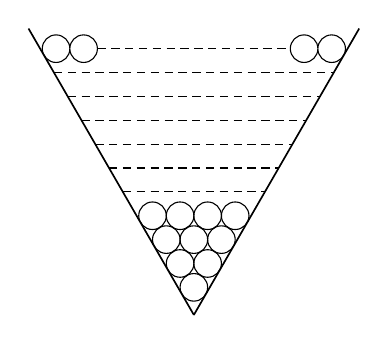
\begin{tikzpicture}[>=latex,scale=0.35]
  \foreach \r in {0,1,2,3}
  {
    \foreach \x in {0,...,\r}
    {
      \draw([xshift=\x cm]120:\r)circle(0.5);
    }
  }
  \draw([xshift=1cm]120:10)circle(0.5)(120:10)circle(0.5);
  \draw([xshift=9cm]120:10)circle(0.5)([xshift=10cm]120:10)circle(0.5);
  \draw[densely dashed]([xshift=1.5cm]120:10)--++(7,0);
  \foreach \x in {4,...,9}
    {\draw[densely dashed]([xshift=-5.77mm]120:\x)--++(\x+1.154,0);}
  \draw[semithick](0,-1)--++(60:12);
  \draw[semithick](0,-1)--++(120:12);
\end{tikzpicture}
\end{document}